%!TEX root = ../thesis_master.tex
%*******************************************************************************
% * Copyright (c) 2006-2013 
% * Institute of Automation, Dresden University of Technology
% * 
% * All rights reserved. This program and the accompanying materials
% * are made available under the terms of the Eclipse Public License v1.0 
% * which accompanies this distribution, and is available at
% * http://www.eclipse.org/legal/epl-v10.html
% * 
% * Contributors:
% *   Institute of Automation - TU Dresden, Germany 
% *      - initial API and implementation
% ******************************************************************************/

Wenn es um Objektmanipulation geht, ist es notwendig, dass der Roboter eine bestimmte Pose in Bezug auf das Ziel einnimmt, bevor der richtige Manipulationsprozess beginnt. In dieser Arbeit wurde ein IBVS-Controller für die Translations- und Lagekinematik eines Flugroboters entwickelt und implementiert.

Unter Verwendung nur von Bilddaten berechnet der Controller die erforderlichen Robotergeschwindigkeiten, um die gewünschte Pose in Bezug auf ein planares Objekt zu erreichen, das auf dem Boden liegt. Zu diesem Zweck werden einige visuelle Merkmale aus den aktuellen und gewünschten Posen berechnet und ihre Differenz wird von einem PID-Regler als Fehler verwendet, der die an die Low-Level-Regler des Fahrzeugs gesendeten Geschwindigkeitsbefehle ausgibt.

Der Controller ist als ROS-Komponente implementiert, sodass er Teil eines modularen Robotersystems sein kann, das auf diesem Framework ausgeführt wird. Schließlich wird das System in einer Simulation eines Quadrotor Flugroboters getestet und verifiziert.

\begin{center}
	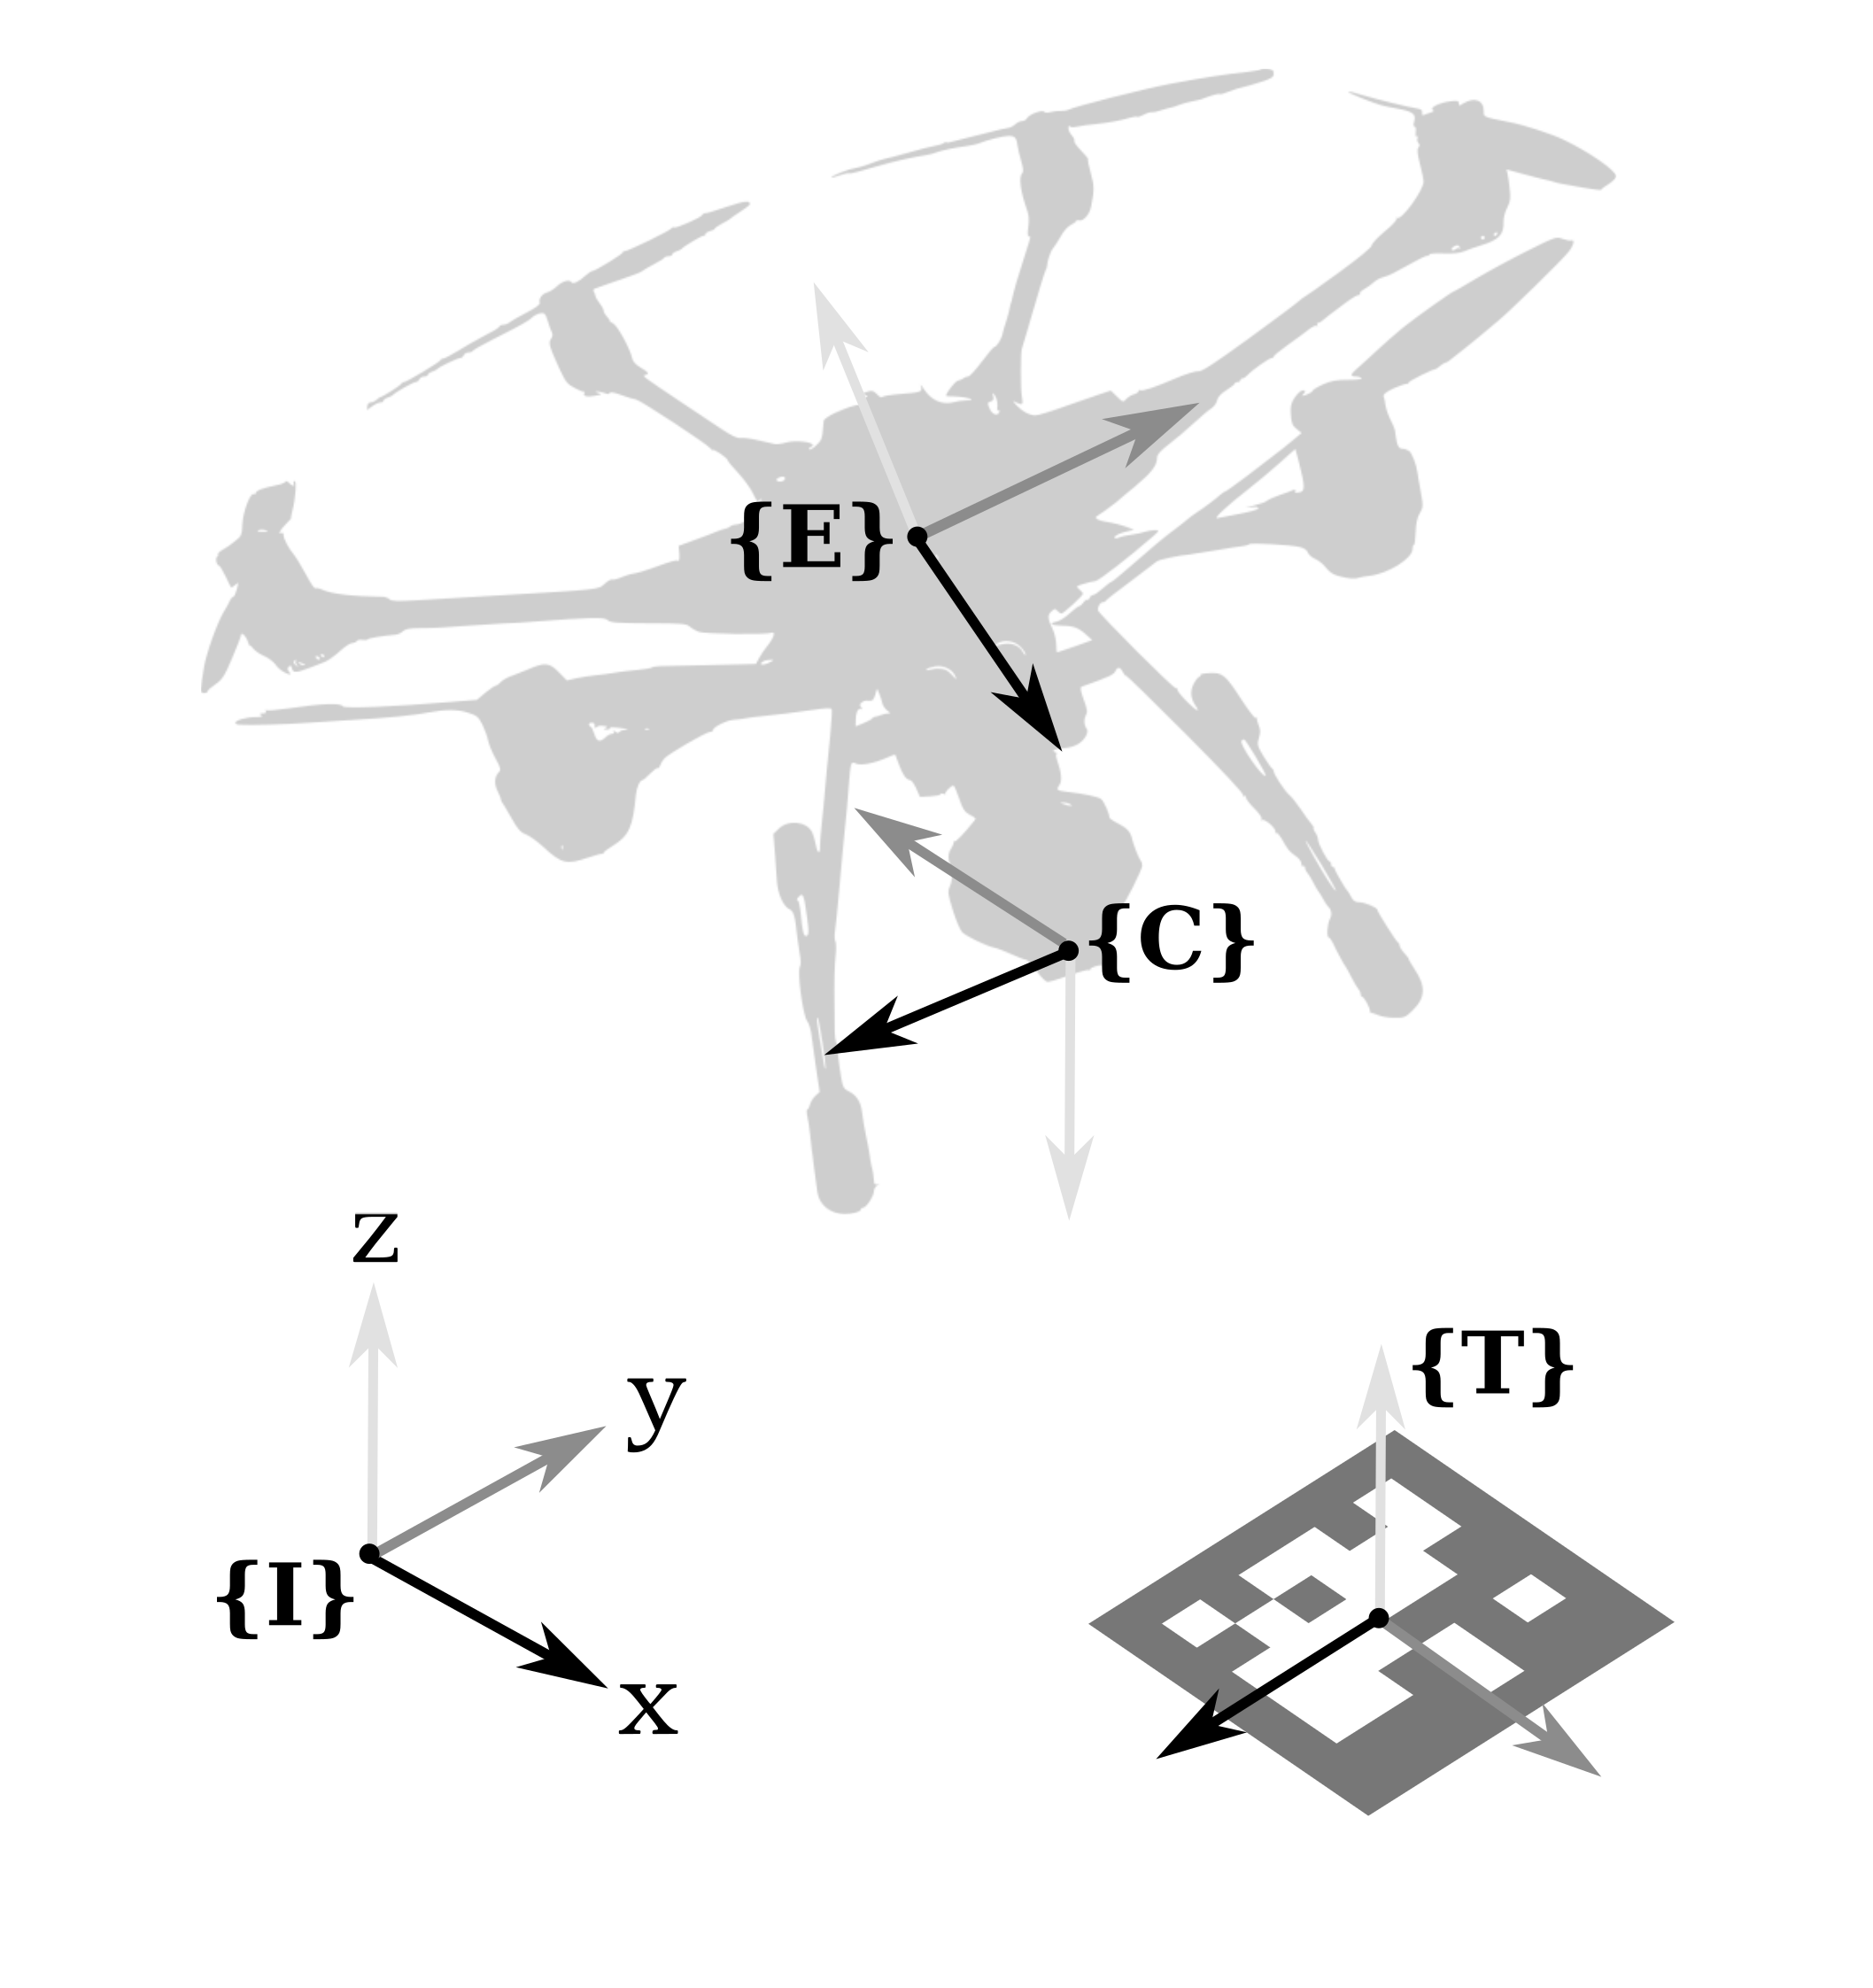
\includegraphics[keepaspectratio, width=5.5cm]{content/frames_bw.png}
\end{center}
